\documentclass{beamer}

% for themes, etc.
\mode<presentation>
{ \usetheme{metropolis} }
%{ \usetheme{Torino} }
%{ \usetheme{boxes} }

\usepackage{times}  % fonts are up to you
\usepackage{graphicx}

% these will be used later in the title page
\title{ALICE MUON Software for run 3}
\author{Sean Murray \\
    Physics \\
    University of Cape Town 
}
\date{July 6, 2016}

% note: do NOT include a \maketitle line; also note that this title
% material goes BEFORE the \begin{document}

% have this if you'd like a recurring outline
\AtBeginSection[]  % "Beamer, do the following at the start of every section"
{
\begin{frame}<beamer> 
\frametitle{Outline} % make a frame titled "Outline"
\tableofcontents[currentsection]  % show TOC and highlight current section
\end{frame}
}

\begin{document}

% this prints title, author etc. info from above
\begin{frame}
\titlepage
\end{frame}

\section{ALICE}

\begin{frame}
\frametitle{ALICE}

  \center{
  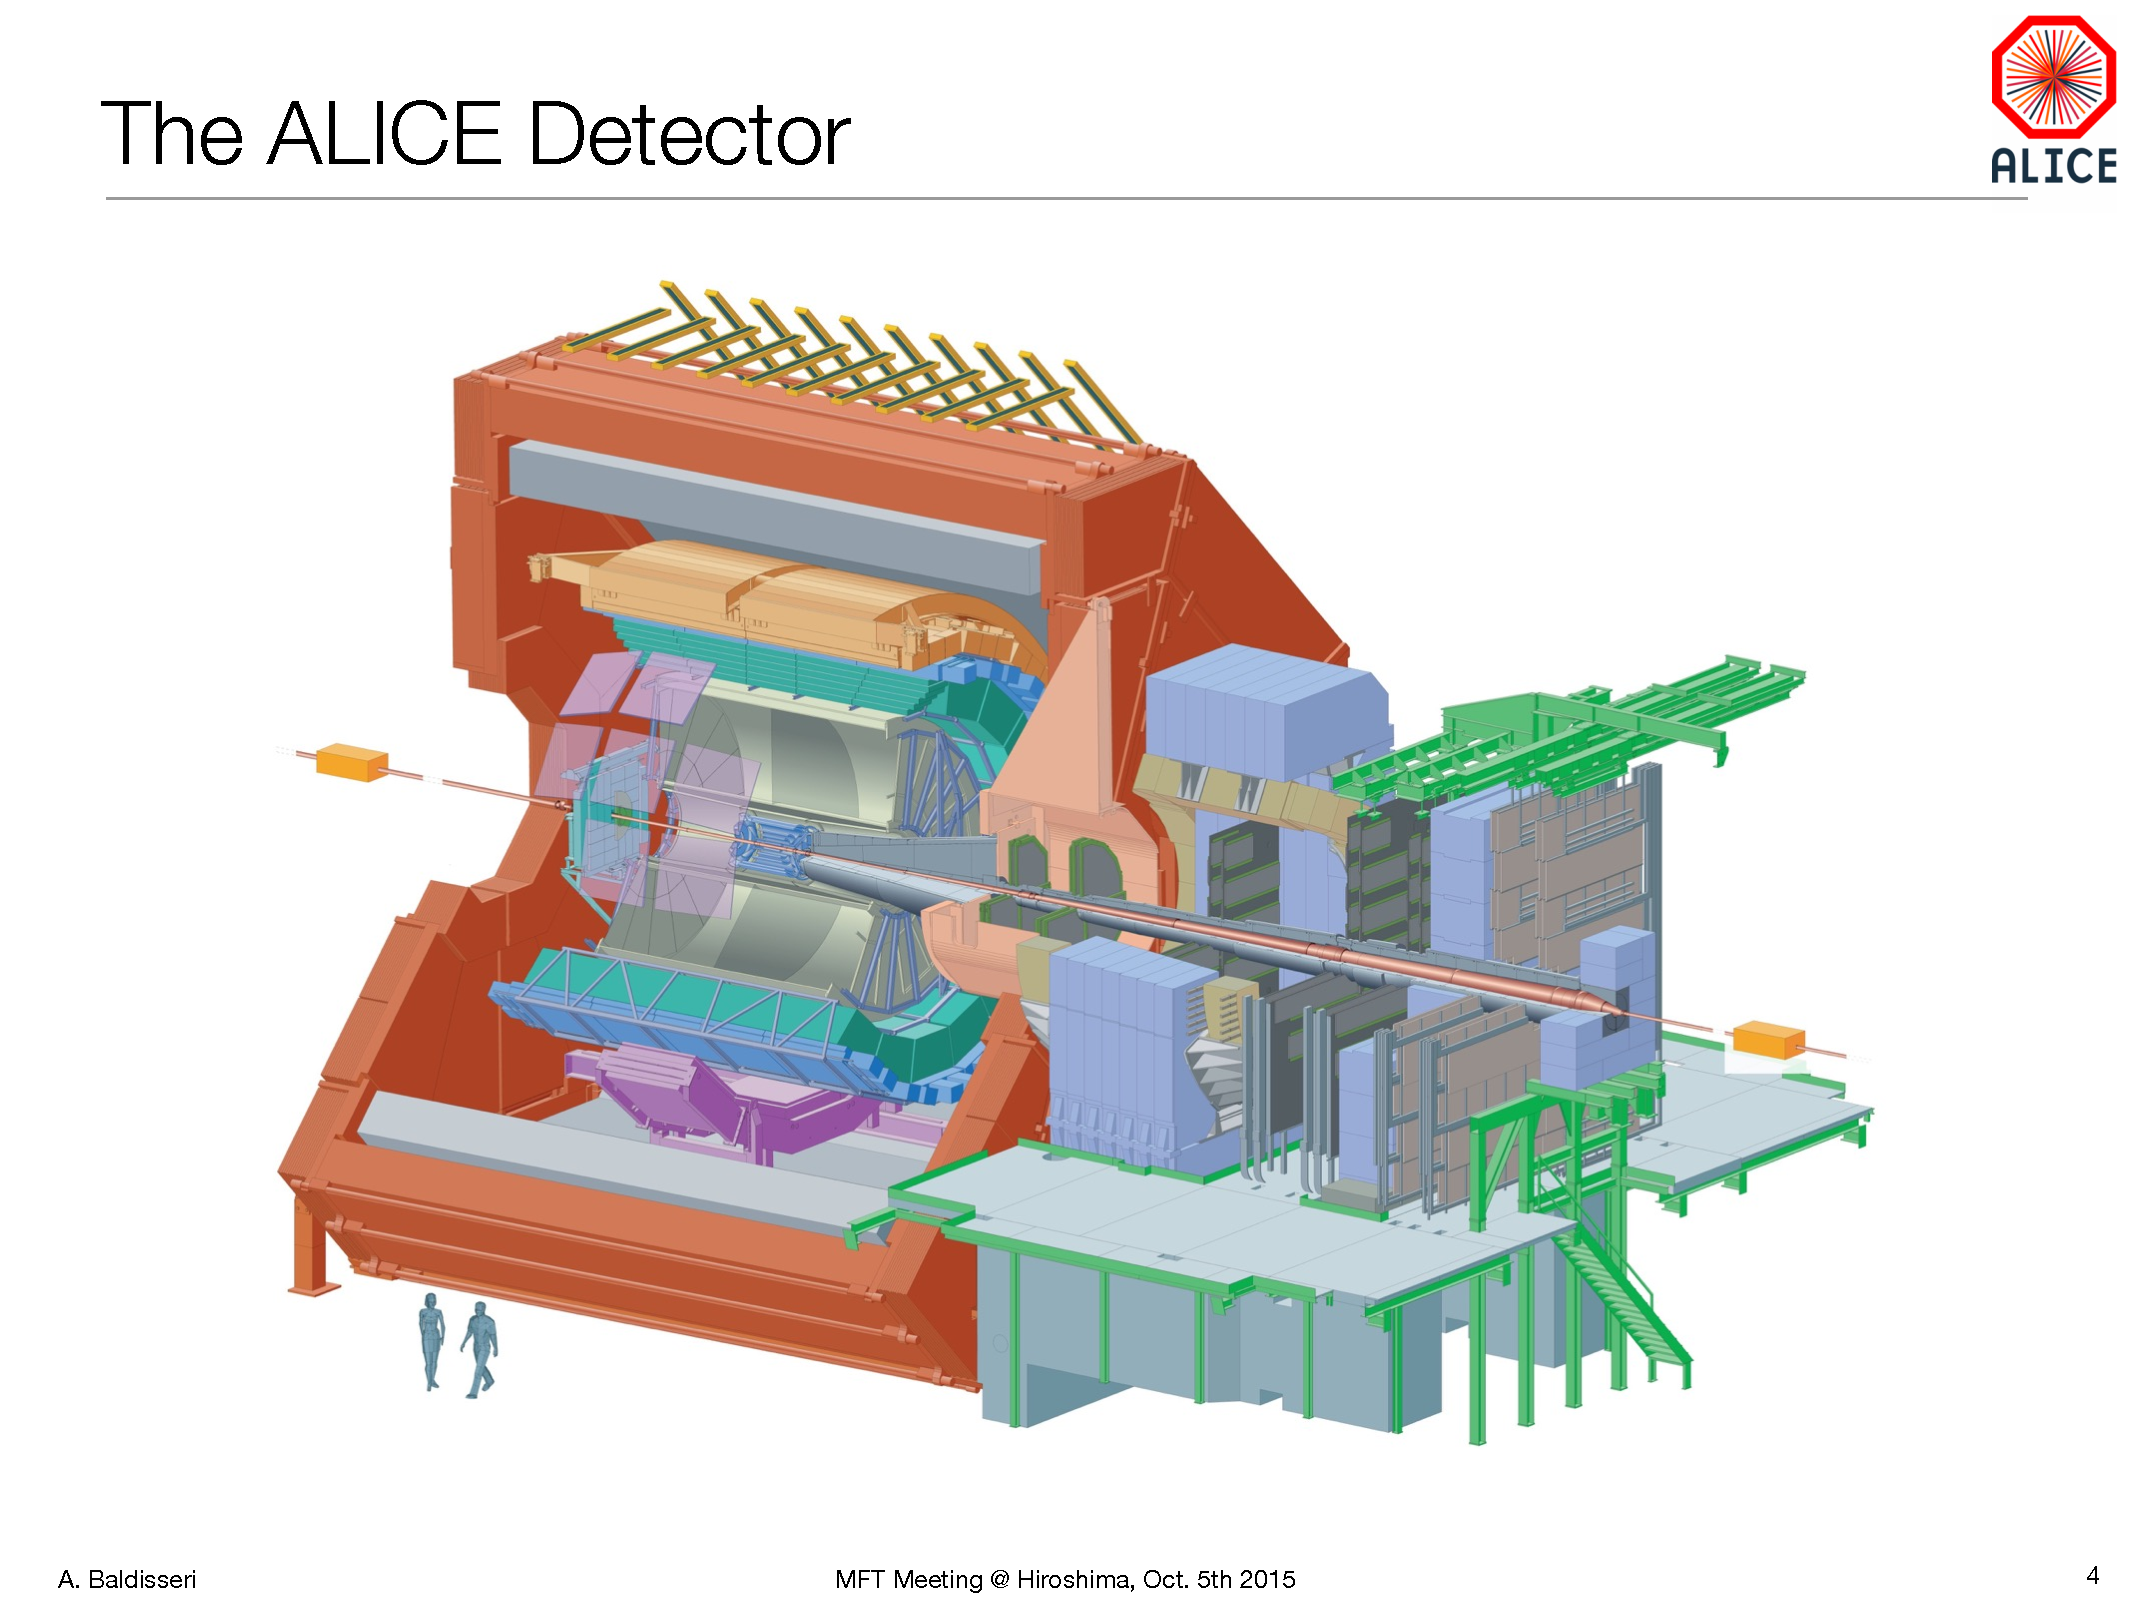
\includegraphics[scale=0.35,trim={5cm 2cm 3cm 4cm},clip]{images/pg_0004.pdf}
  }
\end{frame}

\begin{frame}
\frametitle{ALICE MUON Arm}
  \center{
  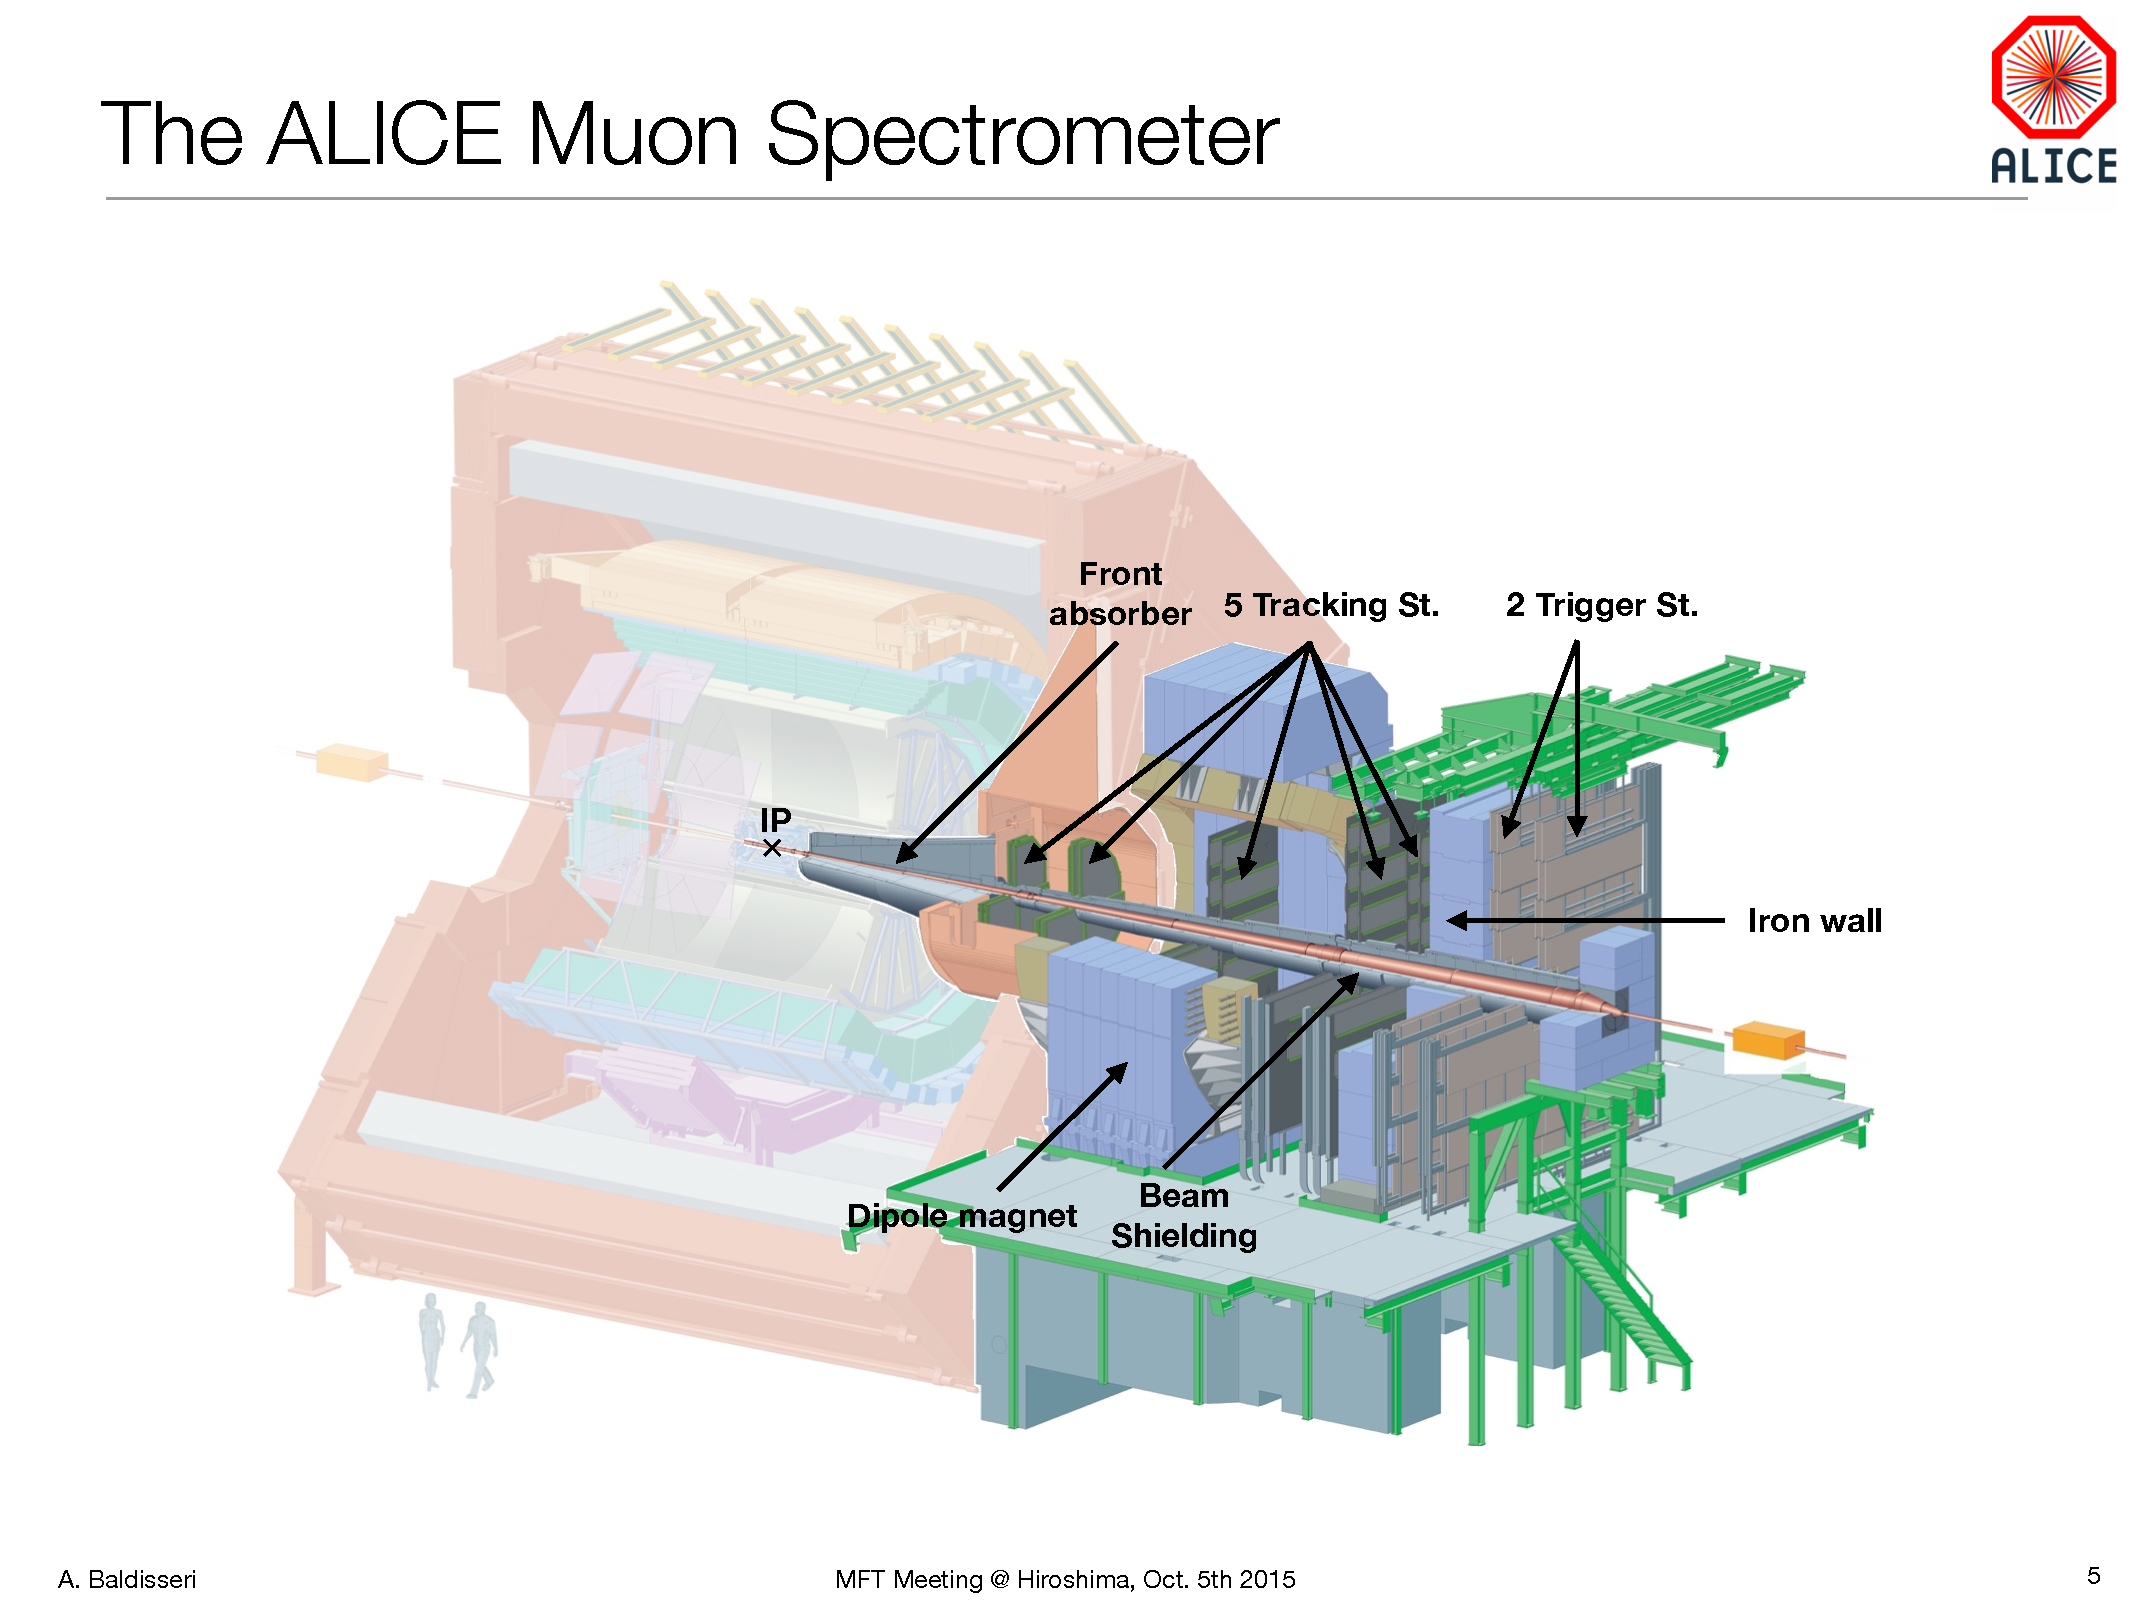
\includegraphics[scale=0.35,trim={3cm 1cm 3cm 4cm},clip]{images/pg_0005.pdf}
  }
\end{frame}

\begin{frame}
  \frametitle{ALICE MUON diagram}

  \center{
  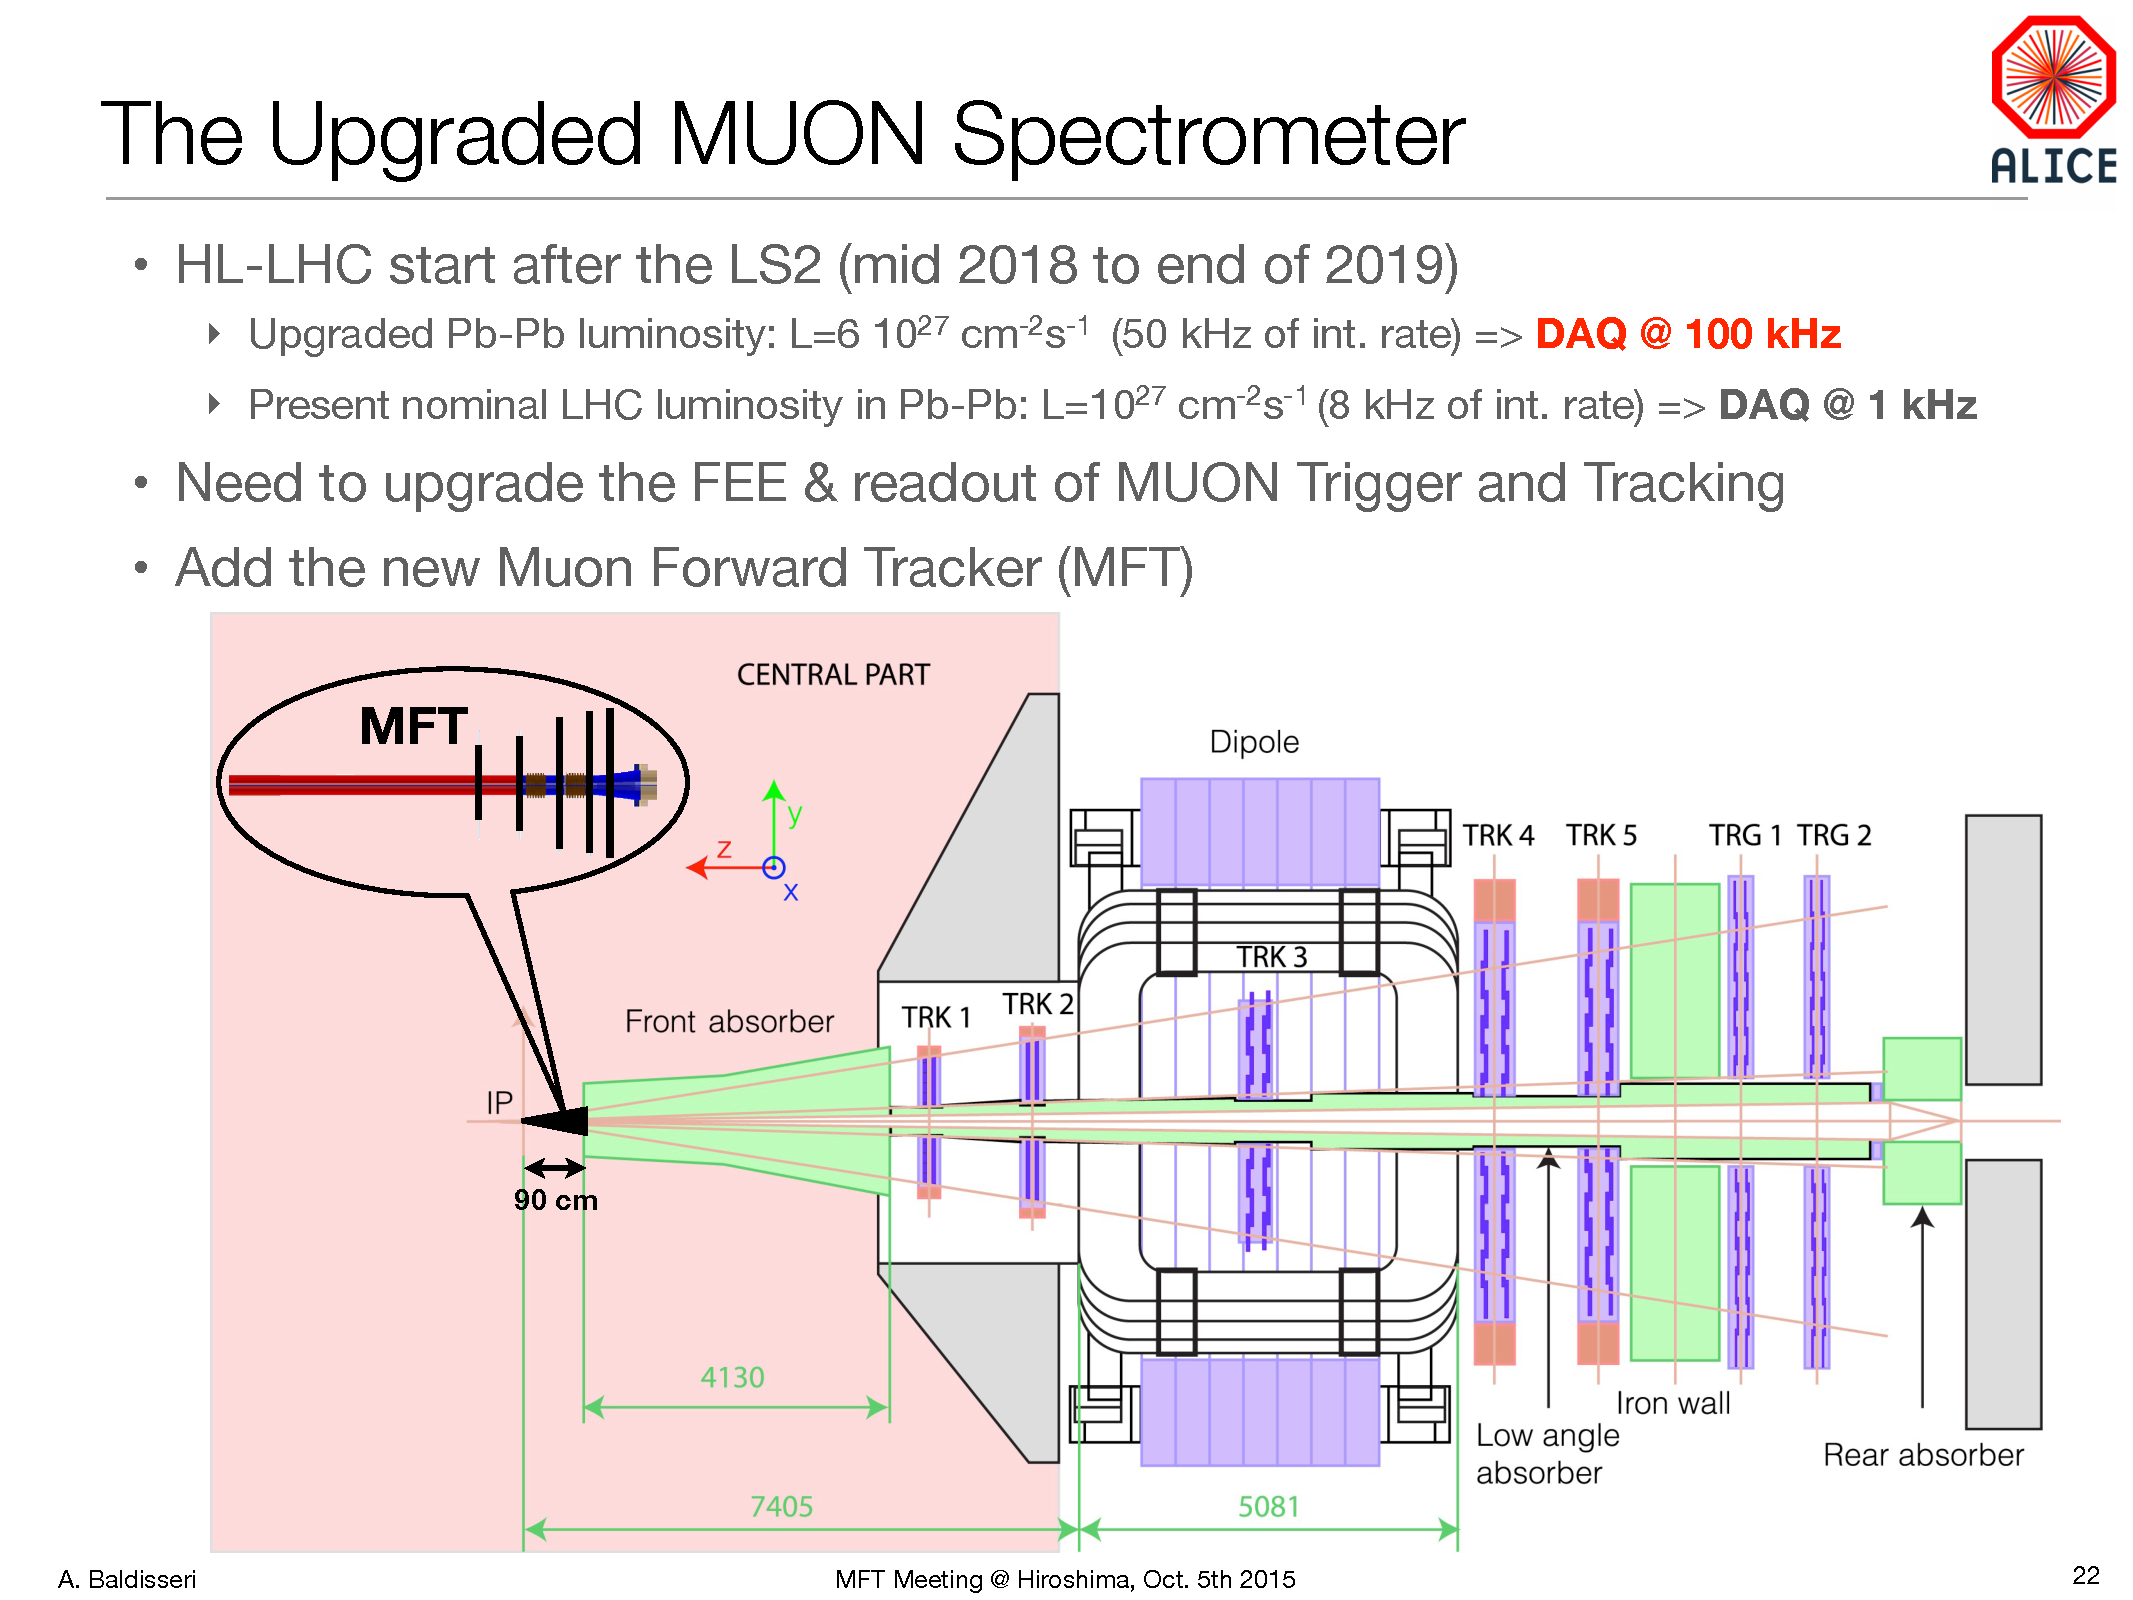
\includegraphics[scale=0.35,trim={2cm 0.75cm 1cm 10cm},clip]{images/pg_0022.pdf}
  }

\end{frame}

\begin{frame}
\frametitle{Detector Structure Station1}
\centering{
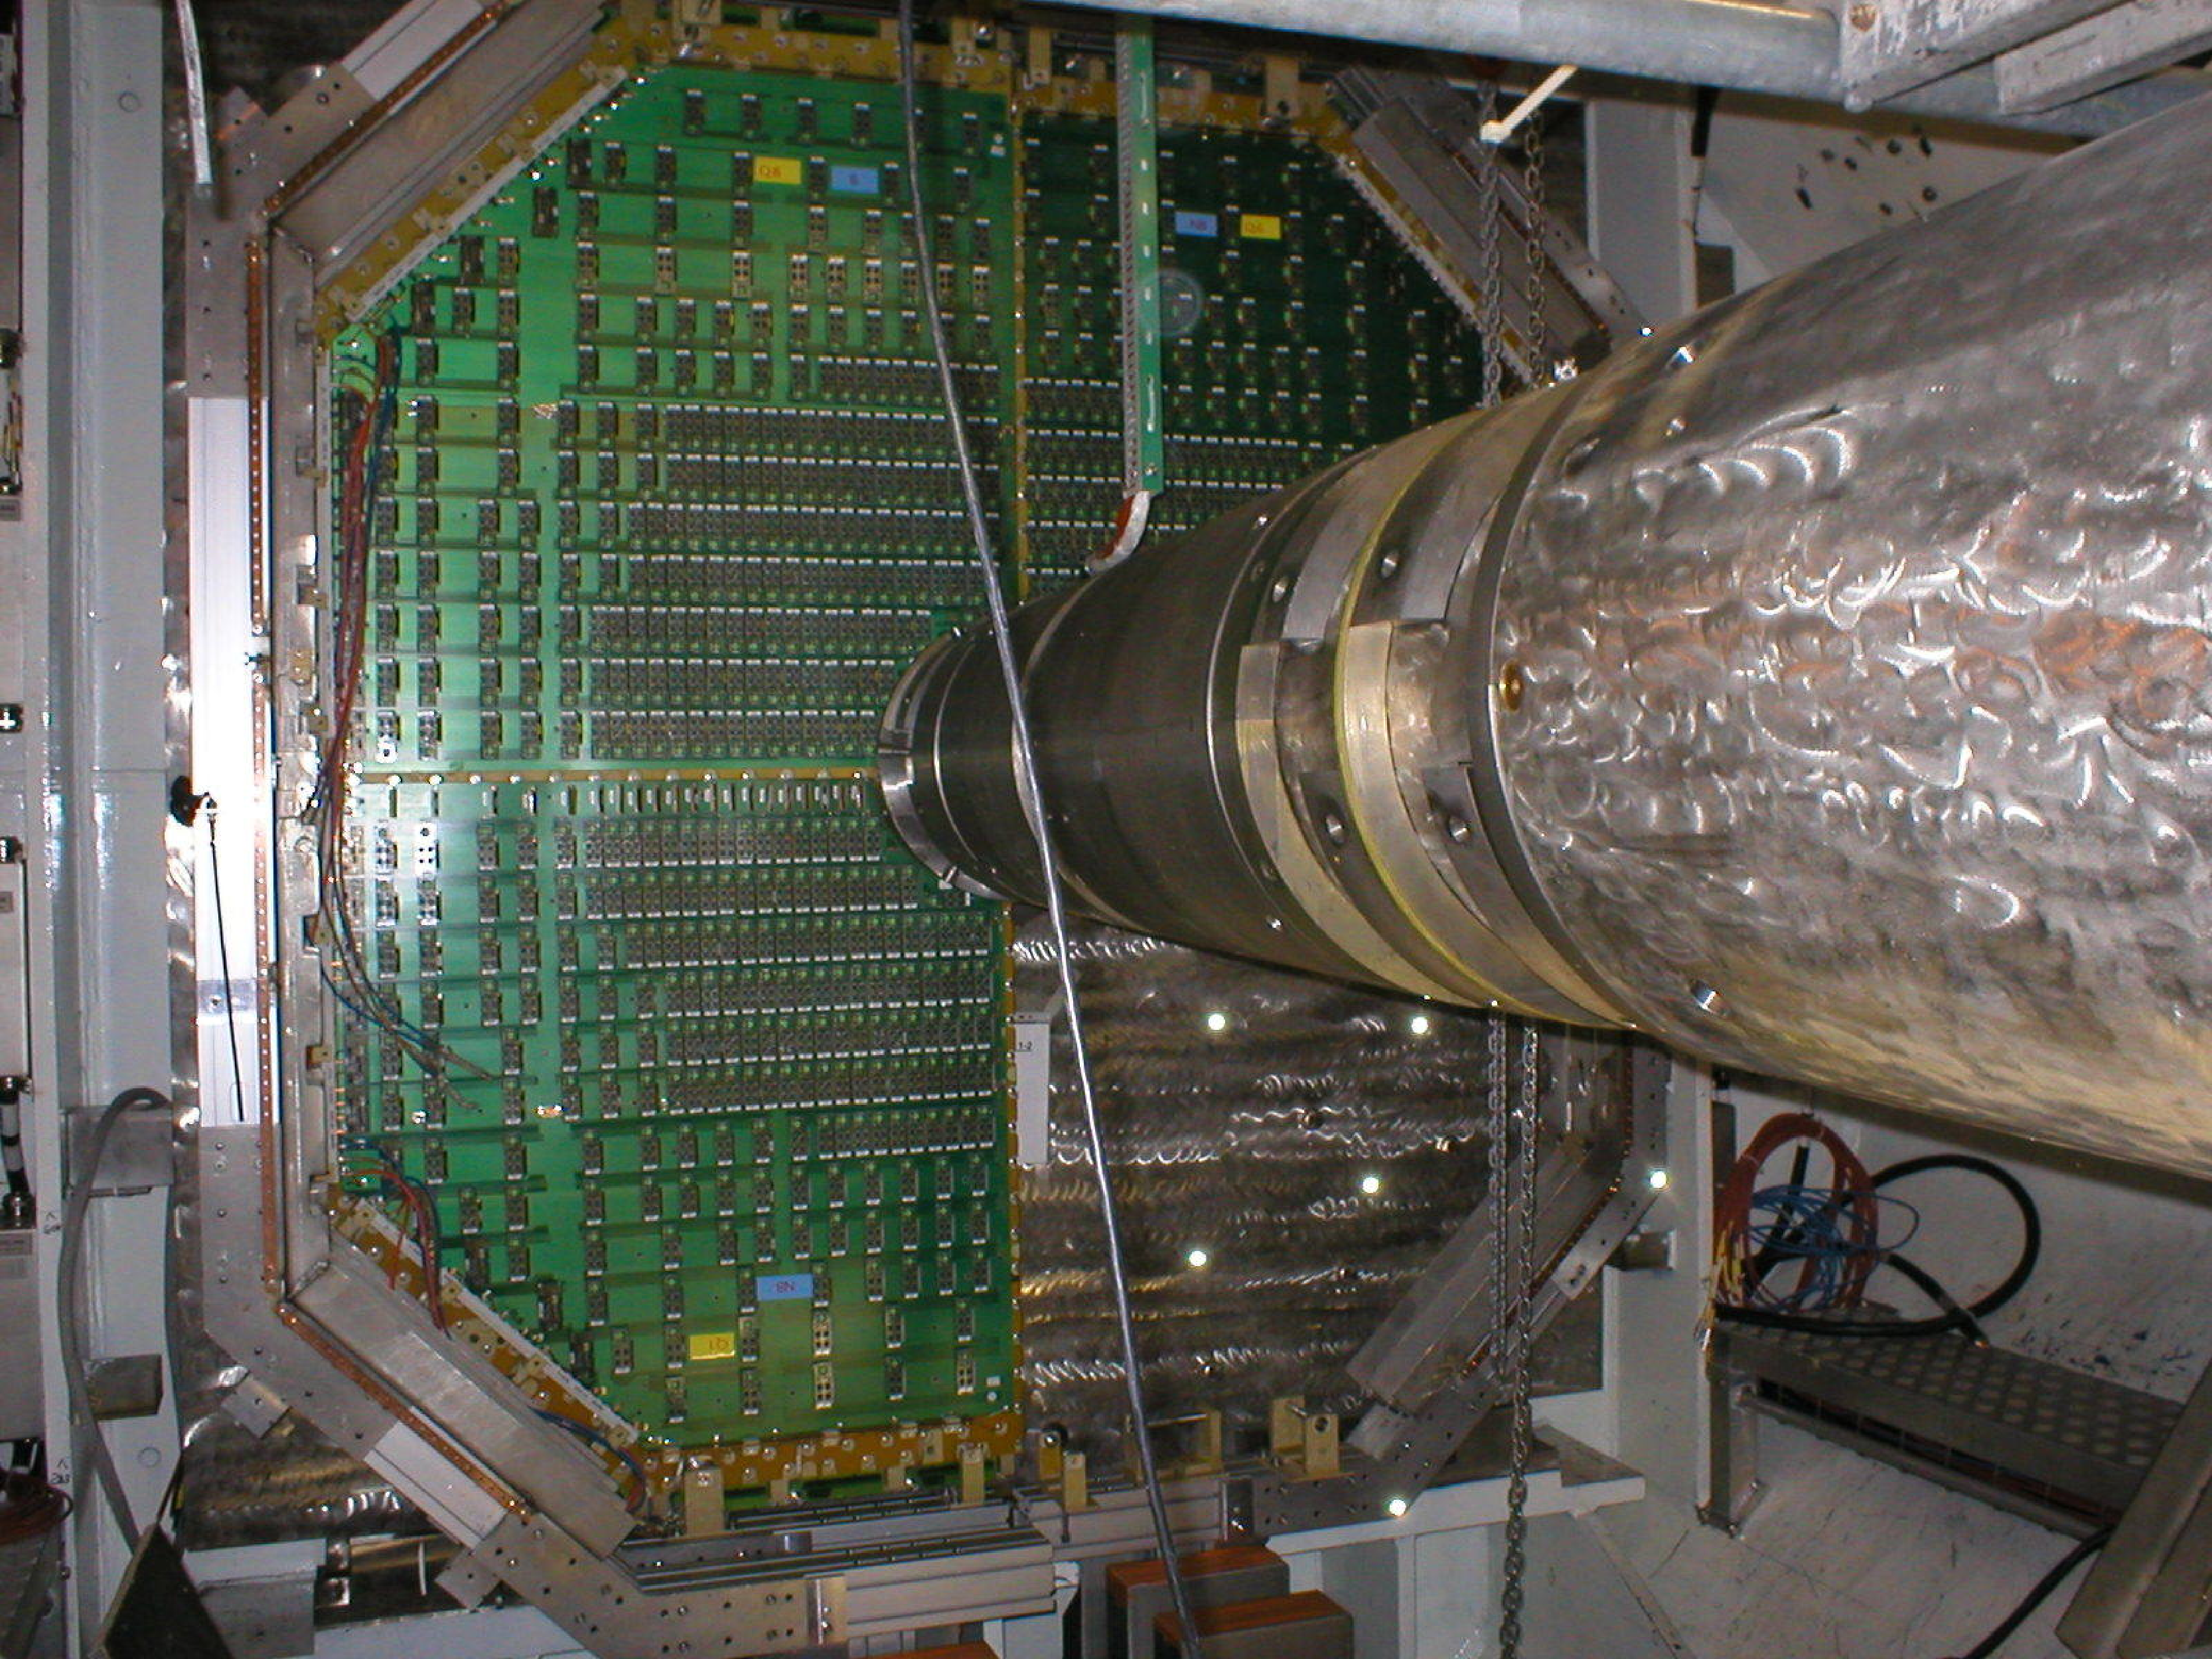
\includegraphics[scale=0.25]{images/MuonStation1.pdf}
} 
\end{frame}

\begin{frame}
\frametitle{Detector Slats}
\centering{
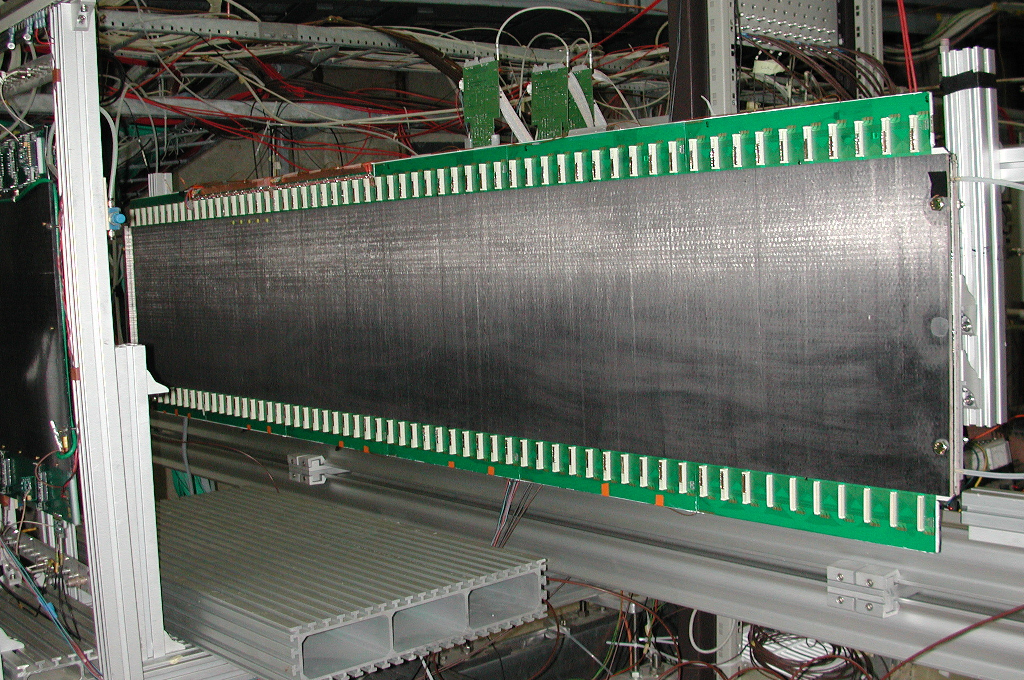
\includegraphics[scale=0.5]{images/MUONSlat.pdf}
} 

\end{frame}

\begin{frame}
\frametitle{Detector Slats in Position}
\centering{
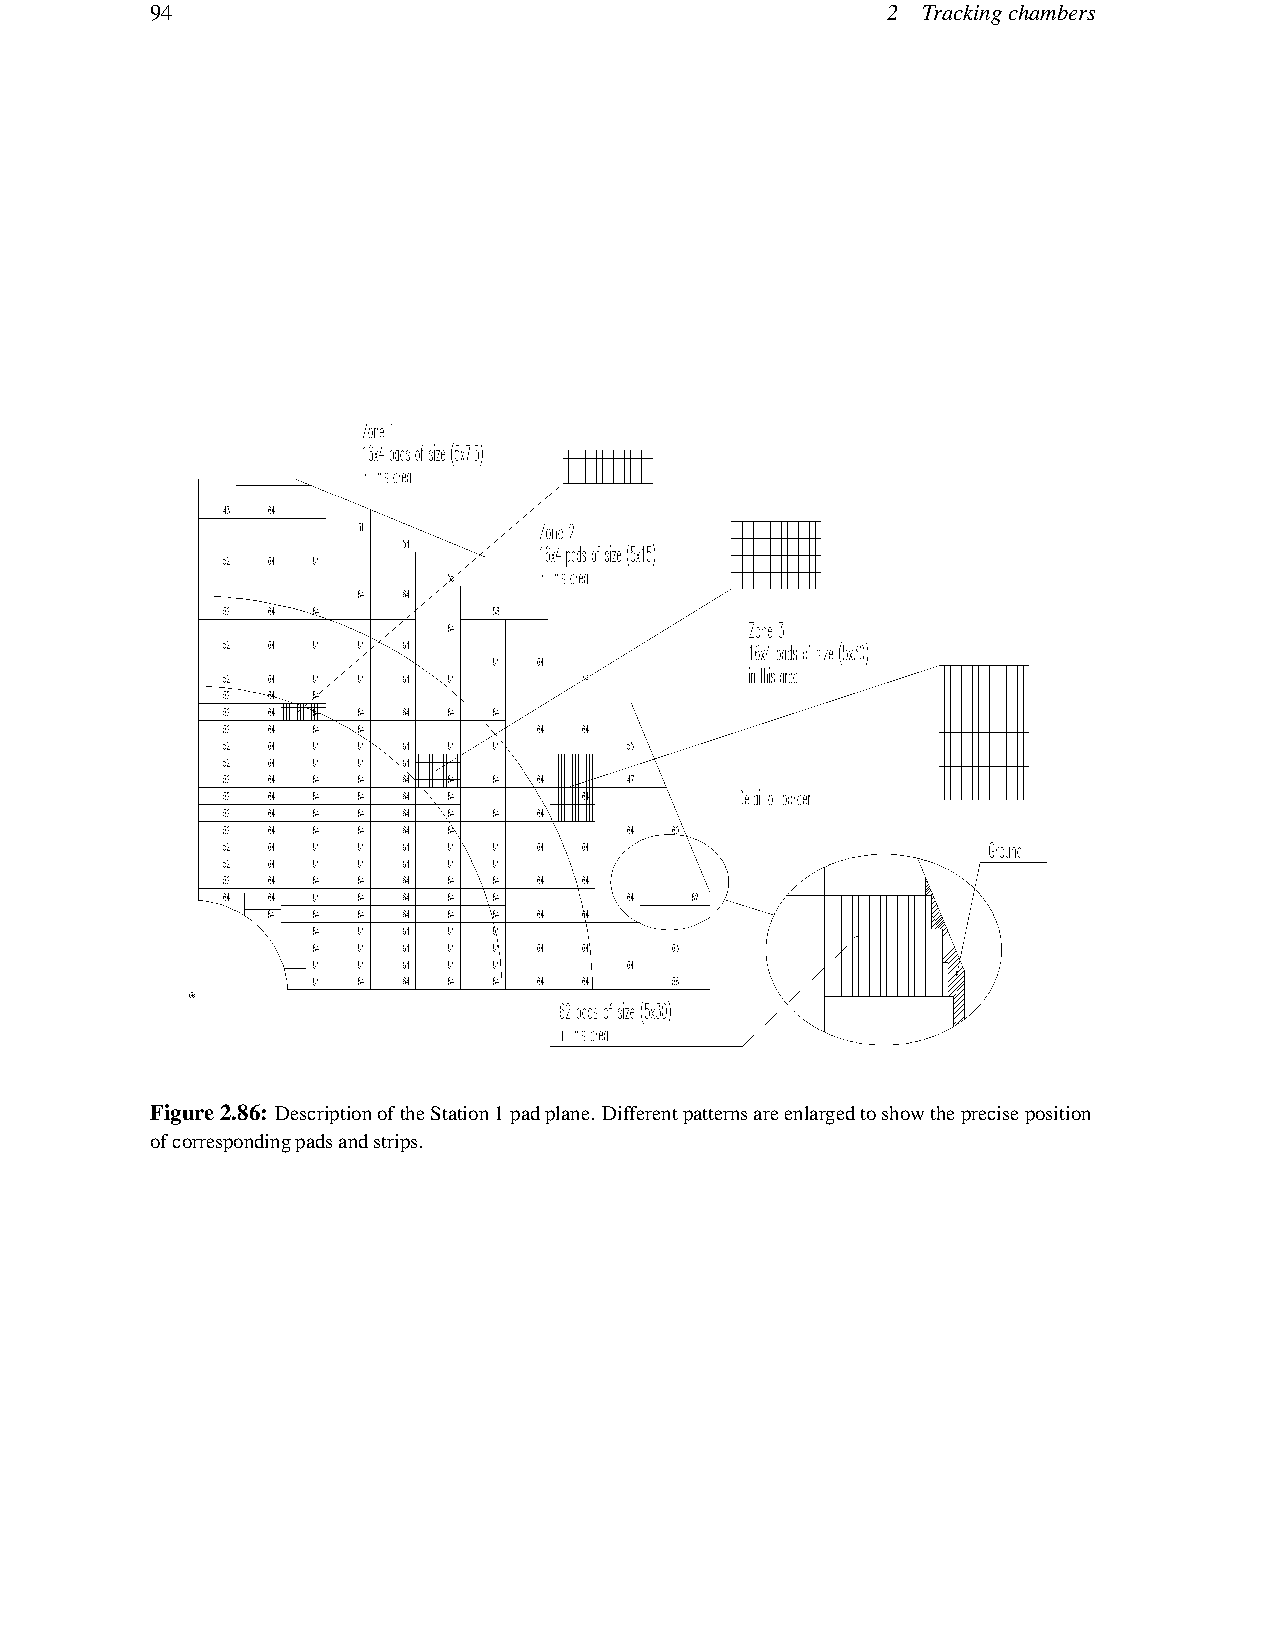
\includegraphics[scale=0.75,trim={2cm 7cm 3cm 7cm},clip]{images/Station1Wires.pdf}
} 

\end{frame}

\section{O2 and Run3}
\begin{frame}
\frametitle{O2 Online/Offline}
hlt daq offline pic

\end{frame}
\begin{frame}
  \frametitle{O2 Farm}
\end{frame}

\section{Current MUON Software}

\begin{frame}
\frametitle{Current MUON Software}


\begin{itemize}
  \item Raw Data Decoding
  \item Raw Data Filtering
  \item Pre Clustering
  \item Clustering
  \item Tracking (MCH)
  \item Tracking (MID)
  \item Track Matching MCH-MID
\end{itemize}
\end{frame}


\begin{frame}
  \frametitle{Time Spent}
\begin{proof}

\begin{tabular}{|l|r|}
  Function & \% Time \\ 
% uncover makes advanced overlay
\uncover<1->{Raw Data Decoding} & \uncover<2->{4}\\
\uncover<3->{Raw Data Filtering} & \uncover<4->{2}\\
\uncover<5->{Pre Clustring} & \uncover<6->{10}\\
\uncover<7->{Clustering} & \uncover<8->{63}\\
\uncover<9->{Tracking MCH} & \uncover<10->{7}\\
\uncover<11->{Tracking MID} & \uncover<12->{6}\\
\uncover<13->{Track matching} & \uncover<14->{8}\\
\end{tabular}\\
\end{proof}

Need more data for broader run (PbPb, pPb, pp) and errors.
\end{frame}

\section{Cluster Finder}

\begin{frame}
\frametitle{What is a cluster finder} 
picture of a couple of clusters.
\begin{itemize}
\item some stuff

\end{itemize}

\end{frame}
\begin{frame}
  \frametitle{Logical Parts}
  \begin{itemize}
    \item Add Virtual pads if necessary  
    \item Find Center of Gravity given maximal pixel
      \item aaa
  \end{itemize}
  \begin{equation}
    X_{ocg}=\frac{\sum_{i=1}^5 X_i Q_i}{Q_i}
  \end{equation}
\end{frame}
\end{document}

